\section{Theoretische Grundlagen}

Zum weiterführenden Verständnis der von uns gewählten Methoden und Ansätze soll im Folgenden die wissenschaftlichen Grundlagen geschaffen werden. Hierfür wird die Annahme fachlicher Qualifikation, durch den/die Leser/in getroffen und vorausgesetzt.

\subsection{Neurobiologische Grundlagen der künstlichen Neuronalen-Netze}
%Fully Corrected
Die grundlegenden Ansätze, Ideen und Inspirationen für künstliche neuronale Netze finden sich wie bei vielen technischen Errungenschaften der Ingenieurwissenschaften in der Natur beziehungsweise der damit verbundenen Wissenschaft des Lebens, der Biologie.\newline
Die Überlegungen zu neuronalen Netzen basieren grundlegend auf neurobiologischen Konzepten. Hierdurch ergibt sich eine große Ähnlichkeit zwischen einem künstlichen Neuron und einer Nervenzelle (biologischen Neuron), dargestellt in  \ref{fig:neuron}.\newline

% Source neuronimage
\begin{figure}[H]
    \centering
    \includegraphics[scale=0.3]{Studienarbeit_F1/images/neuron.png}
    \caption[Vereinfachte Darstellung eines Neurons]{Vereinfachte Darstellung eines Neurons\footnotemark}
    \label{fig:neuron}
\end{figure}
\footnotetext{\citet{neuronimage}}
Mit Blick auf die Funktionsweise empfängt das Neuron die Erregung über ein weitverzweigtes System von Dendriten. Die Dendriten sind dabei Verbindungsschnittstelle zu den Synapsen beziehungsweise Axonterminalen vorgelagerter Neuronen. Die empfangenen Reize werden in Form von elektrischen Signalen über den Zellkörper (Soma) zum sogenannten Axonhügel weitergeleitet, der Verbindungsstelle des Axons mit dem Zellkörper. Sie gliedern sich dabei in Abhängigkeit von den auslösenden Synapsen in exzitatorische postsynaptische Potenziale (EPSP) mit einer erregenden Wirkung und inhibitorische postsynaptische Potenziale (IPSP) mit einer hemmenden Wirkung.\zitat{4f}{neuronbasics}\newline
Der Axonhügel bildet den zentralen Punkt der Summation der verschiedenen Signale. Hier werden die verschiedenen vielen ankommenden postsynaptischen Potenziale entsprechend ihrer erregenden oder hemmenden Wirkung aufsummiert und lösen gegebenenfalls ein Aktionspotenzial aus. Die Auslösung des Aktionspotenzials erfolgt nach dem sogenannten \glqq Alles-oder-nichts\grqq-Prinzip. Hierzu muss von der Überlagerung beziehungsweise Summation der ankommenden Signale ein gewisser Schwellenwert erreicht werden, welcher bei Überschreitung ein elektrisches Aktionspotenzial am Axonhügel auslöst. Die Form und der Verlauf des Aktionspotenzials sind dabei bei jeder Auslösung identisch und somit unabhängig vom Grad der Überschreitung des Schwellenwertes.\newline
Dieses Aktionspotenzial wird über eine Nervenfaser, das sogenannte Axon zu weiteren nachfolgenden Nervenzellen weitergeleitet.\zitat{22ff}{introductiontoneuralnetworks}\newline
Das Axon ist dabei von sogenannten Myelinscheiden umgeben, die in regelmäßigen Abständen von den ranvierschen Schnürringen unterbrochen sind. Diese nur bei Wirbeltieren vorkommenden Neuronenbestandteile ermöglichen durch die isolierende Wirkung der Myelinscheiden eine sogenannte saltatorische Erregungsleitung, welche sich durch eine besonders schnelle Übertragungsgeschwindigkeit des Aktionspotenzials gegenüber der kontinuierlichen Erregungsleitung auszeichnet.\zitat{1}{signalconduction}\newline
Die schlussendliche Übertragung der Erregung zwischen den Nervenzellen erfolgt in den meisten Fällen durch die Ausschüttung von chemischen Botenstoffen, den sogenannten Neurotransmittern an den Axonterminalen. Diese Ausschüttung wird durch die Ankunft des das Axon entlang gewanderten Aktionspotenzials ausgelöst. Diese Neurotransmitter erzeugen an den Dendriten der nachfolgend angeordneten Nervenzellen wieder eine erregende oder hemmende Wirkung.\zitat{22ff}{introductiontoneuralnetworks}\newline
Auf eine tiefer gehende Erläuterung biologischer Neuronen, insbesondere hinsichtlich ihrer biochemischen Funktionsweise, wird an dieser Stelle verzichtet, da dies für den Rahmen dieser Arbeit nicht zielführend wäre. %%Hier kann evtl. auch noch ein Buchverweis eingefügt werden, wenn man es für notwendig hält. So nachdem Schema: Auf eine genauere Erläuterung der Funktionsweise biologischer Neuronen wird, mit Verweis auf weiterführende Literatur [Verweise], verzichtet, da dies für den Rahmen dieser Arbeit nicht zielführend wäre.
\subsection{Künstliches Neuron}
\label{künstliches_neuron}
%Fully Corrected
Die Grundstruktur und theoretische Funktionsweise eines künstlichen Neurons, welches die Grundlage künstlicher neuronaler Netze bildet, orientiert sich in großem Maße an seinem biologischen Äquivalent. Seine Funktions- beziehungsweise Arbeitsweise kann anhand dem in \ref{fig:technicalneuron} abgebildeten Modell des Selbigen nachvollzogen und veranschaulicht werden.
%aineuron
\begin{figure}[H]
    \centering
    \includegraphics[scale=0.2]{Studienarbeit_F1/images/NeuronModel.png}
    \caption[Schaubild eines künstlichen Neurons]{Schaubild eines künstlichen Neurons\footnotemark}
    \label{fig:technicalneuron}
\end{figure}
\footnotetext{\citet{aineuron}}
Ein solches künstliches Neuron kann eine Vielzahl von Eingabewerten besitzen, welche entsprechend \ref{fig:technicalneuron} mit $x_1$ bis $x_n$ bezeichnet werden. Diese Eingabewerte werden mit zugehörigen Kantengewichten verrechnet, die das Maß des Einflusses der jeweiligen Eingabe auf das Neuron festlegen. Diese Gewichte werden mit $w_{1j}$ bis $w_{nj}$ bezeichnet.\\
Mit Blick auf das biologische Neuron lässt sich dieser Aspekt grundlegend mit den verschiedenen Arten der postsynaptischen Potenziale vergleichen.\zitat{5f}{neuronbasics}\\
Die Übertragungsfunktion erfüllt die Anforderung der Berechnung der Netzeingabe $net_j$. Dieser Wert repräsentiert dabei die Kumulierung aller Eingaben in Kombination mit den entsprechenden Gewichten. Mathematisch lässt sich dieser Sachverhalt beschreiben mit folgender Formel:\\
\begin{subequations}
    \begin{align}
    net_j = \sum\limits_{i=1}^n x_i \cdot w_{ij}
    \end{align}
Mit Blick auf das biologische Äquivalent ist dies mit der zuvor erläuterten Funktion des Axonhügels zu vergleichen.\\
Die Aktivierungsfunktion $\varphi$ ermittelt auf Grundlage der Netzeingabe $net_j$ und eines Schwellenwertes $\theta_j$ eine resultierende Aktivierung $o_j$. Demnach ergibt sich die Aktivierung $o_j$ eines Neurons und damit der Wert, der an potenziell nachfolgende Neuronen weitergeleitet wird, entsprechend:\\
    \begin{align}
        o_j = \varphi(net_j + \theta_j)
    \end{align}
Für die Aktivierungsfunktion $\varphi$ können verschiedene grundlegende Funktionen verwendet werden.\zitat{29ff}{introductiontoneuralnetworks} Nachfolgend werden die grundlegenden Arten von Aktivierungsfunktionen dargestellt. %Fully Corrected
\begin{itemize}
    \item \textbf{Heaviside-Funktion}:\\
    Die nachdem britischen Mathematiker und Physiker \glqq Oliver Heaviside \grqq benannte Funktion ist die grundlegendste Aktivierungsfunktion eines künstlichen Neurons. Alternative Bezeichnungen sind Treppen-Funktion oder Step-Funktion.\\
    Sie nimmt für alle Werte $v$ für die gilt $v < 0$ den Wert $0$ an, während sie für alle $v \geq 0$, den Wert $1$ an nimmt.
    Sie ergibt sich somit entsprechend
    \begin{align}
    \varphi(v) = \begin{cases}
            0 : v < 0 \\
            1 : v \geq 0
            \end{cases}
    \end{align}
    \begin{figure}[h]
        \centering
    \begin{tikzpicture}
    \begin{axis}[
    xmin = -1, xmax=1,
    ymin = -0.1, ymax=1.1,
    xtick={-1,-0.5,0,0.5,1}]
    \addplot[color=red]
    coordinates {(-1,0)(-0.5,0)(-0.00000001,0)(0,1)(0.5,1)(1,1)};
    \addlegendentry{Heaviside}
    \end{axis}
    \end{tikzpicture}
    \caption{Schaubild der Heaviside-Funktion}
    \end{figure}\\
    %ToDo, den Plot noch ein bisschen hübscher machen. ->"Bisschen mehr Luft um das Schaubild drum rum und die Linie des Graphen auch etwas dicker
    %ToDo Hier noch ein matplotlib Schaubild einfügen
    Die Verwendung dieser Aktivierungsfunktion erzeugt bei einem künstlichen Neuron ein Verhalten, welches dem \glqq Alles-oder-nichts\grqq-Verhalten seiner biologischen Vorbilder gleicht. Das künstliche Neuron erzeugt nur dann eine Aktivierung, wenn der Schwellenwert erreicht ist. Auch ist der Wert der Aktivierung nicht vom Grad der Überschreitung des Schwellwertes abhängig, was dem bei jeder Auslösung identischen Verlauf des Aktionspotenzials entspricht. Die Aktivierung bleibt entweder aus oder ist in vollem Umfang vorhanden, es existiert dabei keine Zwischenstufe.\\
    Der Gradient der Heaviside-Funktion ergibt sich über den gesamten Definitionsbereich zu null. Dadurch ist es nicht möglich, ein neuronales Netz nach dem Konzept der Fehler-Backpropagation zu trainieren. Diese Eigenschaft sorgt dafür, dass der Einsatz der Heaviside-Funktion in der Praxis meist vermieden wird.\zitat{2}{ImprovingNeuralNetworks} 
    Ein gängiger Anwendungsfall dieser Funktion findet sich Kontext der Single-Output-Networks im Zuge der binären Klassifikation.\zitat{3}{2021ReviewandComparison}%Keine Ahnung ob das richtig zitiert ist
    \item \textbf{Sigmoid-Funktion:}\\
    Eine weitverbreitete und in der Praxis häufig verwendete Aktivierungsfunktion stellt die sogenannte Sigmoid-Funktion dar. Weitere gängige Bezeichnungen sind logistische Funktion oder Quetschfunktion.\zitat{5f}{nwankpa2018activation}
    Sie stellt einen typischen Vertreter der \glqq S\grqq-förmigen Aktivierungsfunktionen dar. Diese zeichnen sich durch ihren nicht linearen Verlauf aus. Die typische Sigmoid-Funktion ist in Abhängigkeit der Eingabewerte $v$ definiert durch:
    \begin{align}
        \varphi(v) = \frac{1}{1+e^{-v}}
    \end{align}
    \begin{figure}[h]
        \centering
    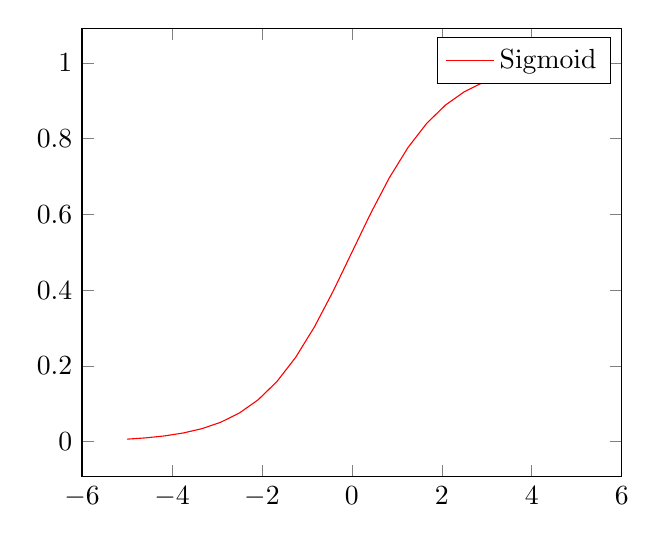
\begin{tikzpicture}
        \begin{axis}[
        ]
            \addplot[color=red]{(1+exp(-x))^(-1)};
            \addlegendentry{Sigmoid}
        \end{axis}
    \end{tikzpicture}
    \caption{Schaubild der Sigmoid-Funktion}
    \end{figure}
    \\
    Bei der Sigmoid-Funktion handelt es sich um eine glatte Funktion, wodurch sie unendlich oft stetig differenzierbar ist.\\
    Sie kann grundsätzlich als Näherung der bei $0$ nicht differenzierbaren Heaviside-Funktion betrachtet werden, welche sich aufgrund ihrer einfachen Differenzierbarkeit innerhalb eines neuronalen Netzes gut verwenden lässt.\zitat{3f}{lederer2021activation} So ergibt sich die Ableitung der Sigmoid-Funktion zu:
    \begin{align}
        \frac{d}{dx}\varphi(v) = \varphi(v) \cdot (1-\varphi(v))
    \end{align}
    In der Praxis wird die Sigmoid-Funktion vor allem zur binären Klassifikation, aber auch zur Simulation von Funktionen eingesetzt. Im Allgemeinen eignet sie sich vor allem zur Anwendung in flachen neuronalen Netzen mit wenigen versteckten Schichten.\\
    Ein weiterer Vorteil der Sigmoid-Funktion neben der stetigen Differenzierbarkeit ist die Abbildung beliebiger Eingabewerte $v$ auf ein begrenztes Intervall von $(0,1)$, wodurch die Aktivierung des einzelnen Neurons innerhalb dieses Intervalls normiert ist.\\
    Dem entgegen steht der Nachteil, dass die Funktionswerte außerhalb des Intervalls [-2,2] kaum auf Änderungen der Eingabewerte reagiert. Somit ist der Gradient der Funktion außerhalb des angegebenen Intervalls sehr klein. Dadurch wird eine effektive Backpropagation erschwert, was dazu führen kann, dass das neuronale Netz sehr langsam oder sogar gar nicht lernt.\zitat{5f}{2021ReviewandComparison} Diese Auswirkung der kleinen Gradienten, welche eine nennenswerte Änderung der Gewichte im Zuge des Lernprozesses verhindert, werden durch eine höhere Anzahl von versteckten Ebenen verstärkt. Dadurch wird die Sigmoid-Funktion als Aktivierungsfunktion für derartige neuronale Netze beziehungsweise ihre versteckten Ebenen ungeeignet.\zitat{5}{nwankpa2018activation}\newpage
    \item \textbf{Rectified-Linear-Unit-Funktion:}\\
    Die Rectified-Linear-Unit-Funktion (ReLU) stellt die derzeit meist verwendete Aktivierungsfunktion innerhalb künstlicher neuronaler Netze dar.\zitat{8}{nwankpa2018activation} Sie wird teilweise als Rampen-Funktion bezeichnet. Sie nimmt für alle Eingabewerte $v$ für die gilt $v \leq 0$ den Funktionswert $0$ an und für alle $v > 0$ den Funktionswert $v$ an.\\
    Somit ist sie formal definiert durch:
    \begin{align}
        \varphi(v) = max(0,v) = \begin{cases}
                            0 \text{, wenn } v \leq 0\\
                            v \text{, wenn } v > 0
        \end{cases}
    \end{align}
    \begin{figure}[h]
    \centering
    \begin{tikzpicture}
    \begin{axis}[
        domain=-3:3,
        ]
        \addplot+[mark=none,red,domain=-3:0] {0};
        \addplot+[mark=none,red,domain=0:3] {x};
        \addlegendentry{ReLU}
    \end{axis}
\end{tikzpicture}
\caption{Schaubild der ReLU-Funktion}
\end{figure}
\\
    Ein wesentlicher Vorteil ist die einfache Implementierbarkeit der ReLU-Funktion und ihrer Ableitung, die sich zur Heaviside-Funktion ergibt. Sie erlauben dabei jeweils eine schnelle und kostengünstige Berechnung.\zitat{8}{lederer2021activation}
    Grund hierfür ist die simple Definition der Funktion, welche im Vergleich zur Sigmoid-Funktion keine Berechnung aufwendiger Divisionen oder Exponenten erfordert, was eine höhere Berechnungsgeschwindigkeit zur Folge hat. Weiterhin erlauben die linearen Eigenschaften der ReLU-Funktion eine effiziente Optimierung mittels Gradientenabstieg.\zitat{8f}{nwankpa2018activation}\\
    %Nachteile Leichtes Overfitting und DyingRelu-Problem, darauf eventuell auch noch eingehen und das erklären
    \item \textbf{Softmax-Funktion:}\\
    Eine weitverbreitete Aktivierungsfunktion aus dem Technologiefeld der neuronalen Netze stellt die Softmax-Funktion dar. Sie dient im Allgemeinen zur Berechnung einer Wahrscheinlichkeitsverteilung über einen Vektor reeler Zahlen. Hierbei erzeugt sie auf Basis des Eingabevektors $v$ der Länge $N$, eine Verteilung deren Einzelbestandteile zwischen $0$ und $1$ liegen und deren Summe sich zu $1$ ergibt.\\
    Sie ist formal definiert durch
    \begin{align}
        \varphi(v_i) = \frac{e^{v_i}}{\sum_{j=1}^{N} e^{v_j}}
    \end{align}
    Die Softmax-Funktion wird im Vergleich zur Sigmoid-Funktion zur multivariaten Klassifikation verwendet, während diese im Bereich der binären Klassifikation angewandt werden kann. Weiterhin wird sie in beinahe in sämtlichen Architekturen neuronaler Netze als Aktivierungsfunktion der Ausgabeschicht verwendet.\zitat{8}{nwankpa2018activation}
    
\end{itemize}
\end{subequations}

\subsection{Lernprozess künstlicher neuronaler Netze}\label{lernprozess}
Wie in Kapitel \ref{künstliches_neuron} erläutert, wird die Verarbeitung der Daten aus der vorherigen Schicht eines neuronalen Netzes im Wesentlichen über die Gewichte gesteuert. Um die Verhaltensweise der Ausgabe in einem Lernprozess zu adaptieren, muss demnach eine Methode zur Anpassung dieser gefunden werden. Für die Erläuterung eines Verfahrens zur Bewerkstelligung dessen wird zunächst die Struktur eines einfachen neuronalen Netzes, des sogenannten \gqq{multilayer perceptron} (MLP) eingeführt. Diese in Abbildung \ref{fig:MLP_structure} dargestellte Architektur umfasst Schichten von parallelen Neuronen, die jeweils vollständig mit ihrer vorherigen und nächsten Schicht verbunden sind. Die beliebig vielen Schichten zwischen der Eingabe- und Ausgabeschicht werden als versteckte Schicht zusammengefasst. Wird jede Kante des Graphen mit einer Gewichtung versehen, ergeben sich für die Aktivierungen eines jeden Neurons die bereits in Kapitel \ref{künstliches_neuron} erarbeiteten Zusammenhänge. Die Komposition mehrerer Schichten mit einer nicht linearen Aktivierungsfunktion für jedes Neuron der versteckten Schicht ermöglicht das Approximieren beliebiger Funktionen mit einer Genauigkeit, die von den genauen Parametern des Netzes abhängt.\footnote{Vgl. \cite{goodfellow_deep_learning} S.164-166} Diese Eigenschaft liefert die Begründung für die Nützlichkeit derartiger neuronaler Netze, da sich eine Vielzahl von Problemen als komplexe Funktionen modellieren lassen. Weiterer Vorteil dieser Architektur ist die Möglichkeit der eleganten mathematischen Beschreibung des Systems. Da sich die Aktivierung eines jeden Neurons aus der Linearkombination der Neuronen-Ausgaben der vorherigen Schicht mit ihren korrespondierenden Kantengewichten zum betrachteten Neuron ergibt, kann die Aktivierung eines einzelnen Neurons als Skalarprodukt implementiert werden. Die Aktivierungen einer gesamten Schicht lassen sich demnach durch mehrere Skalarprodukte der Ausgaben der vorherigen Schicht mit den Gewichten für alle gesuchten Neuronen berechnen. 
\begin{figure}[h]
    \centering
    \includegraphics[scale=0.2]{Studienarbeit_F1/images/Neural_Network_Structure.png}
    \caption{Neuronenstruktur eines MLP}
    \label{fig:MLP_structure}
\end{figure}
Das Bilden von Skalarprodukten eines Vektors mit mehreren anderen Vektoren und das Sammeln der Ergebnisse in einem neuen Vektor ist mathematisch nichts anderes als eine Matrizenmultiplikation. Die Vorwärtspropagierung einer Eingabe in das Netz um eine Schicht lässt sich damit effizient als Matrizenmultiplikation mit anschließender, komponentenweiser Anwendung der Aktivierungsfunktion im Ergebnisvektor implementieren. In Matrixschreibweise ergibt sich die folgende Darstellung:
\begin{subequations}
    \begin{align}
        \label{eq:feedforward_matmul}
        \begin{bmatrix}
            w_{1,1} & w_{2,1} & \cdots & w_{n, 1}\\
            w_{1,2} & w_{2,2} & \cdots & \vdots\\
            \vdots & \vdots & \ddots & \vdots\\
            w_{1, m} & \cdots & \cdots & w_{n, m}
        \end{bmatrix}
        \cdot
        \begin{bmatrix}
            o_{i,1}\\
            \vdots\\
            o_{i,n}
        \end{bmatrix}
        =  
        \begin{bmatrix}
            a_{j, 1}\\
            \vdots\\
            a_{j, m}
        \end{bmatrix}
    \end{align}
    \begin{align}
        \label{eq:feedforward_activation}
        \begin{bmatrix}
            \varphi(a_{j, 1})\\
            \vdots\\
            \varphi(a_{j, m})
        \end{bmatrix} 
        =
        \begin{bmatrix}
            o_{j, 1}\\
            \vdots\\
            o_{j, m}
        \end{bmatrix}
    \end{align}
\end{subequations}
Eine Zeile in der Gewichtsmatrix repräsentiert die Gewichte aller Kanten, die zu einem Neuron der nächsten Schicht hinführen, während alle Spalten die Kantengewichte von einem Neuron der vorherigen Schicht hinweg darstellen. Durch die Multiplikation der Outputs der vorherigen Schicht \(i\) ergeben sich die Aktivierungen der nächsten Schicht \(j\), welche durch die komponentenweise Anwendung der nicht linearen Aktivierungsfunktion \(\varphi\) zu den Outputs der Schicht \(j\) werden.\\
Aus diesem Schema der Vorwärtsverarbeitung muss nun eine Methode zur Anpassung der Gewichte infolge eines Lernbeispiels abgeleitet werden, da nur so eine für das daliegende Problem passende Funktionsapproximation erreicht werden kann.
Für diesen Ansatz wird zunächst ein Sollwert bei der Ausgabe des Netzes benötigt. Dieser repräsentiert bei gegebener Eingabe in das Netz das final gewünschte, also korrekte Ergebnis. Die Abweichung vom Sollwert zum Istwert liefert eine Metrik zur Beurteilung der Performance des Netzes und kann verwendet werden, um die Gewichte in solch einer Weise anzupassen, dass der Wert der Fehlerfunktion minimiert wird. Der hierfür verwendete Algorithmus ist als \gqq{stochastic gradient descent} bekannt. Kern der Überlegung ist es, dass das Finden eines Tiefpunktes der Fehlerfunktion darüber implementiert werden kann, dass die Änderungsrate des Fehlers in Abhängigkeit der einzelnen Gewichte über die Anwendung der Kettenregel berechnet wird. Die Ableitungen werden in einem Vektor zusammengetragen und repräsentieren den Gradienten der Fehlerfunktion in Abhängigkeit der Gewichte. Der Gradient zeigt stets in die Richtung des stärksten Anstiegs eines Skalarfelds, somit resultiert aus der Änderung der Gewichte in Richtung des negativen Gradienten eine Annäherung an einen Tiefpunkt, der Fehler wird also minimiert. Das analytische Ermitteln der Ableitungen nach den Gewichten wird im Folgenden am Beispiel eines Ausgabewertes des Netzes illustriert. Die Ausgabe eines Neurons berechnet sich im allgemeinen Fall nach \ref{eq:feedforward_matmul} und \ref{eq:feedforward_activation} aus der Verkettung von zwei Funktionen, nämlich aus der gewichteten Summe aus den vorherigen Aktivierungen und der Anwendung der Aktivierungsfunktion. Zusätzlich muss die Anwendung der Fehlerfunktion nach der Ausgabeschicht bedacht werden. Ist also die nötige Anpassung des Gewichtes zwischen dem ersten Neuron der vorletzen und dem ersten Neuron der letzten Schicht gesucht, muss der folgende Ausdruck berechnet werden:
\[\frac{\partial E}{\partial w_{ij}} = \frac{\partial E}{\partial o_j} \cdot \frac{\partial o_j}{\partial a_j}\cdot \frac{\partial a_j}{\partial w_{ij}}\]
In Prosa lässt sich der Term insofern erklären, dass zunächst die Fehlerfunktion nach der Neuronenausgabe, dann die Neuronenausgabe nach der Aktivierungsfunktion und zuletzt die Aktivierung des Neurons nach dem gewünschten Gewicht abgeleitet wird. Es resultiert das Verhältnis der Änderung in der Fehlerfunktion zu einer Änderung des relevanten Gewichtes. Theoretisch kann diese Kette an Kompositionen bis zur Eingabeschicht des Netzes zurückverfolgt werden, was für die Ableitung nach den sich dort befindenden Gewichten auch praktiziert wird. Für Gewichte, welche sich in einer früheren Schicht befinden, müssen verschiedene \gqq{Wege} durch das Netz addiert werden, da so ein Gewicht die Fehlerfunktion über mehrere Neuronen beeinflusst.\footnote{Vgl. \cite{goodfellow_deep_learning} S.200 - 213}
Die Details dieser Berechnungen lassen sich beispielsweise in \cite{goodfellow_deep_learning} nachlesen und sind im Wesentlichen triviale weitere Betrachtungen, die auf denselben Ansatz der Anwendung der Kettenregel zur Rückverfolgung der Verbindungen des Netzwerkes zurückgehen.
Moderne Bibliotheken\footnote{Bekannte Beispiele sind PyTorch oder Tensorflow} für die Entwicklung neuronaler Netze sind im Kern Programmierhilfen, die das Definieren von Schichten vereinfachen und die relevanten Ableitungen automatisch berechnen.

\subsection{Diskrete Eventsimulation}
% Fully corrected
Die Möglichkeit einer Simulation durch das Erstellen eines geeigneten Modells zur Analyse birgt umfassende Vorteile gegenüber der reinen Observierung des realen Systems. Beispielsweise enthält der Prozess des Aufbauens des Modells bereits das Potential, die Zusammenhänge im System genauer zu verstehen, aber auch die Notwendigkeit für Details zu erkennen. Weiter erlaubt das Verwenden eines Modells die kontinuierliche Wiederholung der Vorgänge im System bei exakt gleichen Verhältnissen sowie das minimale Anpassen von Parametern, um deren Auswirkungen im untersuchten System umfassender zu verstehen. In diesem Fakt zeichnet sich auch ab, dass das Beeinflussen des Systems in einem Modell leichter fällt als in einer realen Umgebung. Ein weiterer Vorteil der Simulation liegt im Umstand der Schnelligkeit, denn die Simulation kann bei Bedarf ohne Verlust von Information schneller abgespielt werden als das reale Vorbild. Optional kann der Ablauf aber auch verlangsamt werden, um somit wiederum Einblicke zu gewinnen, welche im echten Umfeld nicht möglich sind.\zitat{}{discrete_event_sim_fishman}
\\\\
Ein methodischer Ansatz, eine Simulation zu erstellen, ist durch die diskrete Eventsimulation beschrieben. Hierbei wird versucht, das reale Modell, welches meist von chronologischer Kontinuität geprägt ist, in zeitlich unabhängige feste Ereignisse zu unterteilen, welche aber trotzdem die originale Reihenfolge beibehalten. Wie bei jeder Simulation bleibt dieser Ansatz aber immer eine Annäherung der Wirklichkeit und es ist bei der Implementation auf den gewählten Detailgrad zu achten. Sollte zu stark auf Details im Modell verzichtet werden, verbessert dies zwar die Laufzeit und die Flexibilität des Modells, dennoch leidet aber die Aussagekraft der Ergebnisse darunter. Um in diesem Fall den korrekten Pfad zu wählen, muss zunächst die Zielsetzung des Modells definiert werden, um darauf abzuleiten, ob das Modell sich entsprechend verhält oder der Abstraktionsgrad zu hoch gewählt worden ist.

\subsection{Formel 1} %Alex
% Fully corrected
Die Formel 1 ist eine seit 1950 existierende Rennserie, welche jährlich stattfindet und Rennen global abhält. Dabei besteht ein Rennwochenende aus verschiedenen Trainings sowie einem Qualifying, um die Startreihenfolge für das darauf folgende Rennen festzulegen. Antreten tun dabei verschiedene Teams, welche entweder direkt von Automobilherstellern betrieben werden oder von Externen mit jeweils zwei Autos mit zugehörigen Fahrern / Fahrerinnen pro Team. Die Entwicklung der Autos erfolgt durch jedes Team selbst in einem vorgegebenen Rahmen von Regularien, welche durch die FIA (Federation Internationale de l’Automobile) dem Veranstalter der Formel 1 bestimmt werden. 
\\\\
Nachfolgend werden einzelne Aspekte der Formel 1 aus der technischen Sicht sowie einige Regularien vorgestellt, welche diese Arbeit maßgeblich beeinflussen und besonders bei der Entwicklung des simulierten Trainingsumfeldes relevant sind überhaupt mit der Realität vergleichbare Ergebnisse zu erhalten. Dabei werden dennoch Vereinfachungen getroffen, deren Behandlung und Implementation nicht im zeitlichen Umfang dieser Arbeit realisierbar sind. Beispielsweise werden Wettereinflüsse vernachlässigt, weshalb diese nicht im Rahmen der Formel 1 weiter beschrieben werden.

\subsubsection{Reifen} %Alex

Seit 2019 stehen den verschiedenen Formel 1 Teams pro Rennwochenende nur drei verschiedene Reifenmischungen zur Verfügung, welche vom italienischen Reifenhersteller Pirelli entwickelt und bereitgestellt werden. Diese unterliegen den Bezeichnungen \glqq Soft\grqq{}, \glqq Medium\grqq{} und \glqq Hard\grqq{} in Relation zur Zusammenstellung der Gummimischung des jeweiligen Reifentyps. Entsprechend der Bezeichnung verhalten sich die Reifen auch im Rennbetrieb, so entspricht der \glqq Soft\grqq{} dem weichsten Reifen der drei Kategorien und erlaubt somit den größten Haftungskoeffizient und damit die beste Traktion. Durch die Weichheit verschleißt dieser Reifen aber wesentlich schneller und muss somit früher wieder gewechselt werden. Diesbezüglich verhalten sich die weiteren Mischungen bis zum \glqq Hard\grqq, welcher besonders langlebig ist aber nur eine begrenzte Rundenzeit erlaubt. Die Reifen entsprechen dabei jedem Rennwochenende einer anderen Mischung, um an die Charakteristiken der jeweiligen Rennstrecke angepasst zu sein. Der Grundgedanke von weich zu harter Mischung bleibt dabei aber erhalten und wird entsprechend nur als solcher kommuniziert.\\
Dabei ist die Gesamt-Anzahl der Reifen pro Auto limitiert, worauf aber weiterführend in dieser Arbeit keine weitere Rücksicht genommen wird.

\subsubsection{Regeln} %Alex
% Fully corrected
Das für diese Arbeit relevante Reglement ist rein durch die Notwendigkeit beschrieben, dass jedes Auto pro Rennen mindestens zwei verschiedene Reifenmischungen fahren muss. Heißt ein Auto, welches auf harten Reifen startet wird disqualifiziert, sollte es auf diesen Reifen das Rennen beenden. Es müssen also mindestens einmal pro Rennen die Reifen gewechselt werden und dabei auch verschiedene Mischungen gefahren werden. Das bedeutet, es darf auch nicht ein ganzes Rennen auf drei Reifensätzen der Mischung "weich" gefahren werden.
Weitere Regeln stehen in keinem direkten Zusammenhang zu dieser Arbeit und können entsprechend vernachlässigt werden.

\subsubsection{Renngeschehen}\label{sec:race_behaviour} %Alex
% Fully corrected
Ein Rennen in der Formel 1 besteht aus einer festen Anzahl an Runden, welche absolviert werden müssen. Wer zuerst die geforderte Rundenzahl erfüllt, gewinnt das Rennen. Die restlichen Plätze werden abhängig von der weiteren Zieldurchfahrt bestimmt. Es gibt zwar zeitliche Limitationen, nach welchen die Rennen unabhängig vom Rundenzähler beendet werden, diese sind aber in dieser Arbeit nicht zu berücksichtigen sowie die Sonderregelung für überrundete Autos.\\\\
Ein Auto braucht für eine Runde eine gewisse Zeit in welcher die Reifen entsprechend durch die Belastung abnutzen. Mit zunehmender Abnutzung der Reifen verlieren diese an Haftungseigenschaften und die Traktion für das Fahrzeug wird schlechter, was zwangsweise zu einer langsameren Rundenzeit führt. Darauf basierend muss ein Auto nach einem Rahmen an Runden wieder an die Box, um den Reifen zu wechseln und somit einen Reifenplatzer zu vermeiden, welcher das Rennen für das jeweilige Fahrzeug beenden könnte. In diesem Umstand liegt der Existenzgrund der Rennstrategie, welche das Ziel besitzt, möglichst vorteilhaft den Boxenstopp einzuplanen, um möglichst wenig Zeit in Bezug zur gesamten Rennzeit zu verlieren.\\\\
Ein besonderer Aspekt, welcher hierbei mit berücksichtigt werden muss, ist der Umstand, dass moderne Formel 1 Autos große Schwierigkeiten beim Verfolgen eines vorausfahrenden Autos haben. Die durch das vorausfahrende Auto verwirbelte Luft reduziert die aerodynamische Effizienz des eigenen Fahrzeugs und reduziert somit die Haftung auf dem Boden. Dies bedeutet eine geringere Kurvengeschwindigkeit und somit eine langsamere Rundenzeit. Sollte dennoch versucht werden, die Geschwindigkeit des vorausfahrenden Fahrzeugs mithalten zu wollen, so muss der eigene Reifen stärker strapaziert werden, was wiederum zu einem schnelleren Verschleiß des Reifens führt. Zudem kann ein Reifen in dieser Situation schneller überhitzen, was wiederum weniger Traktion und schnelleren Verschleiß bedeutet. Das vorausfahrende Fahrzeug sollte also möglichst schnell überholt werden, um das eigene Rennen nicht weiter zu kompromittieren.\\\\
Beim Überholen ist zusätzlich zu beachten, dass das vorausfahrende Auto meist nicht freiwillig die Position abgibt. Dies bedeutet, dass zwischen den Autos ein Kampf um die Position stattfindet, welcher besonders durch die zur Verfügung stehende Traktion eines Autos bestimmt wird. So fällt es einem Auto auf frischen weichen Reifen verhältnismäßig leichter an einem Fahrzeug auf alten harten Reifen vorbeizukommen, als im Falle von gleicher Bereifung für beide Fahrzeuge. In diesem Fall kann es auch dazu führen, dass der Überholvorgang nicht erfolgreich bleibt und das hintere Auto nicht schneller die Runde vollenden kann als das Auto davor.

\subsection{Polynominale Regression}\label{sub: polynominal_regression}
% Fully corrected
Die polynominale Regression oder auch \gqq{Polynominal Least Square Fit} beschreibt ein Verfahren, um näherungsweise eine Funktion zu generieren, welche bestmöglich zu einem gegebenen Datensatz passt. Dabei versucht das Verfahren die Varianz zwischen den späteren angenäherten Werten pro Datensatz und den tatsächlichen Werten der Eingangsdaten zu minimieren.\\
Der grundlegende Ansatz einer Regression basiert auf der allgemeinen Gleichung einer Funktion, welche in Gleichung \ref{default_func_term} dargestellt ist. Hierbei sind alle Parameter $a$ unbekannt und müssen entsprechend dem gewünschten Grad der Funktion auf Basis der gegebenen Datenpunkte bestimmt werden.
\begin{equation}\label{default_func_term}
    y = a_k*x^k + a_{k-1} * x^{k-1} + ... + a_1*x + a_0
\end{equation}
Ein Ansatz, dieses Problem zu lösen ist, jede Gleichung aufzustellen, welche das System erfüllen muss und anschließend nach den gesuchten Parametern aufzulösen. Dies bedeutet, jeden einzelnen gegebenen Punkt in die allgemeine Funktionsgleichung einzusetzen und das resultierende Gleichungssystem zu lösen. Hierbei kann auf die Matrix-Schreibweise eines Gleichungssystems zurückgegriffen werden. Dies dient der Übersichtlichkeit und erleichtert die methodische Lösung des Systems bei großen Datenmengen.

\begin{subequations}
    \begin{align}\label{eq: approch_poly_reg}
    \begin{bmatrix}
    1 & x_1 & \cdots   & x_1^k \\ 
    1 & x_2  & \cdots  & x_2^k \\ 
    \vdots  & \vdots  & \ddots  & \vdots \\ 
    1 & x_n & \cdots  & x_n^k
    \end{bmatrix}
    \begin{bmatrix}
    a_0 \\
    a_1 \\
    \vdots \\
    a_k
    \end{bmatrix}
    =
    \begin{bmatrix}
    y_0 \\
    y_1 \\
    \vdots \\
    y_k
    \end{bmatrix}
    \end{align}
\\
Zur allgemeinen Lösung der Gleichung \ref{eq: approch_poly_reg} muss auf die von Roger-Moore beschriebene Pseudo-Inverse zurückgegriffen werden, welche es erlaubt, eine Division durch eine nicht quadratische Matrix durchzuführen. Hierzu wird die transponierte Matrix von links auf beide Seiten der Gleichung multipliziert, um somit die Gleichung weiterhin zu erfüllen, dabei aber eine quadratische Matrix als Produkt der zu invertierenden Matrix und ihrer Transponierten zu erzeugen. Diese Matrix kann dann durch ihre quadratischen und symmetrischen Eigenschaften invertiert werden und somit zur Lösung der Gleichung genutzt werden.\zitat{}{polynomial_regression}
%\cite{polynomial_regression}

    \begin{align}\label{eq: pseudo_inverse_poly_reg}
    \begin{bmatrix}
    1 & 1 & \cdots & 1 \\ 
    x_1 & x_2  & \cdots  & x_n \\ 
    \vdots  & \vdots  & \ddots  & \vdots \\ 
    x_1^k & x_2^k & \cdots  & x_n^k
    \end{bmatrix}
    \begin{bmatrix}
    1 & x_1 & \cdots   & x_1^k \\ 
    1 & x_2  & \cdots  & x_2^k \\ 
    \vdots  & \vdots  & \ddots  & \vdots \\ 
    1 & x_n & \cdots  & x_n^k
    \end{bmatrix}
    \begin{bmatrix}
    a_0 \\
    a_1 \\
    \vdots \\
    a_k
    \end{bmatrix}
    =
    \begin{bmatrix}
    1 & 1 & \cdots & 1 \\ 
    x_1 & x_2  & \cdots  & x_n \\ 
    \vdots  & \vdots  & \ddots  & \vdots \\ 
    x_1^k & x_2^k & \cdots  & x_n^k
    \end{bmatrix}
    \begin{bmatrix}
    y_0 \\
    y_1 \\
    \vdots \\
    y_k
    \end{bmatrix}
    \end{align}
    
    \begin{align}\label{eq: solution_poly_reg}
    \begin{bmatrix}
    n & \sum_{i=1}^{n} x_i & \cdots & \sum_{i=1}^{n} x_i^k \\ 
    \sum_{i=1}^{n} x_i & \sum_{i=1}^{n} x_i^2  & \cdots  & \sum_{i=1}^{n} x_i^{k+1} \\ 
    \vdots  & \vdots  & \ddots  & \vdots \\ 
    \sum_{i=1}^{n} x_i^{k} & \sum_{i=1}^{n} x_i^{k+1} & \cdots  & \sum_{i=1}^{n} x_i^{2k}
    \end{bmatrix}
    \begin{bmatrix}
    a_0 \\
    a_1 \\
    \vdots \\
    a_k
    \end{bmatrix}
    =
    \begin{bmatrix}
    \sum_{i=1}^n y_i \\
    \sum_{i=1}^n x_i y_i \\
    \vdots \\
    \sum_{i=1}^n x_i^k y_i
    \end{bmatrix}
    \end{align}
\end{subequations}
\\
In die resultierende Gleichung \ref{eq: solution_poly_reg} können jetzt die entsprechenden Summen der Datenpunkte eingesetzt und abschließend durch die Multiplikation mit der Inversen nach dem Vektor a aufgelöst werden. Die resultierenden Parameter in die allgemeine Funktionsgleichung \ref{default_func_term} eingesetzt ergeben dann die gewünschte Funktionsgleichung, welche nun die Datenmenge bestmöglich repräsentiert.\\
Das diese Lösung eine bestmögliche Näherung der Datenmenge darstellt, wird durch eine andere Herleitung der Gleichung \ref{eq: solution_poly_reg} offensichtlich. Hierbei werden Residuen genutzt. Ein Residuum beschreibt in der numerischen Mathematik den Abstand einer Funktion zu einem Punkt bei identischem Wert $x$.
\begin{subequations}
    \begin{align}\label{eq: def_residual}
        r = y_{dot} - y_{func}
    \end{align}
Dieser Ansatz basiert darauf, die allgemeine Funktionsgleichung \ref{default_func_term} in die allgemeine Form der Residuen einzusetzen und aufzusummieren, um damit die \gqq{Fitness} der gesamten Funktion auf die gesamte Menge der Datenpunkte untersuchen zu können. Aufgrund des Umstandes, dass die resultierenden Residuen positiv wie negativ sein können und somit sich in Summe wieder annullieren würden, werden die Ergebnisse quadriert, um dieses Problem zu umgehen, wie beispielsweise auch bei der Berechnung der Standardabweichung in der Statistik.
    \begin{align}\label{eq: complete_residuals_function}
        R^2 = \sum_{i=1}^n [y_i - (a_k*x_i^k + a_{k-1} * x_i^{k-1} + ... + a_1*x_i + a_0)]^2
    \end{align}
Um eine möglichst gut passende Funktion zur Datenmenge zu erhalten, muss der resultierende Wert $R^2$, welcher dann die gesamte \gqq{Fitness} der gewünschten Funktion repräsentiert, minimiert werden. Dies kann methodisch über die partielle Ableitung nach jedem einzelnen Parameter $a_k$ erreicht werden. 
    \begin{align}
        \frac{\partial(R^2)}{\partial(a_k)} = -2 \sum_{i=1}^n[y-(a_0+a_1x+...+a_k x^k)] = 0
    \end{align}
Entsprechend ergibt sich für jedes $a_k$ eine eigene Gleichung, welche zur Minimierung gleich null gesetzt werden muss. Eine anschließende Umformung und Darstellung des Gleichungssystems als Matrix ergibt dieselbe Gleichung \ref{eq: solution_poly_reg}.\zitat{}{math_poly_reg}
\end{subequations}